\centerline{\bf \Huge Сложные радоси}

\problem{1} В треугольнике $ABC$ провели высоты $AA_1$, $BB_1$ и $CC_1$, точка $H$ --- ортоцентр.\\
(a) Пусть $A'$ --- точка пересечения $B_1C_1$ и $BC$. Точки $B'$ и $C'$ определяются аналогично. Докажите, что точки $A'$, $B'$ и $C'$ лежат на одной прямой.\\
(b) На сторонах $BC$, $CA$ и $AB$ выбраны произвольные точки $K$, $L$, $M$ соответственно. Докажите, что общие хорды окружностей, построенных на отрезках $AK$, $BL$ и $CM$ как на диаметрах, пересекаются в точке $H$.

\begin{figure}[h]
    \begin{center}
        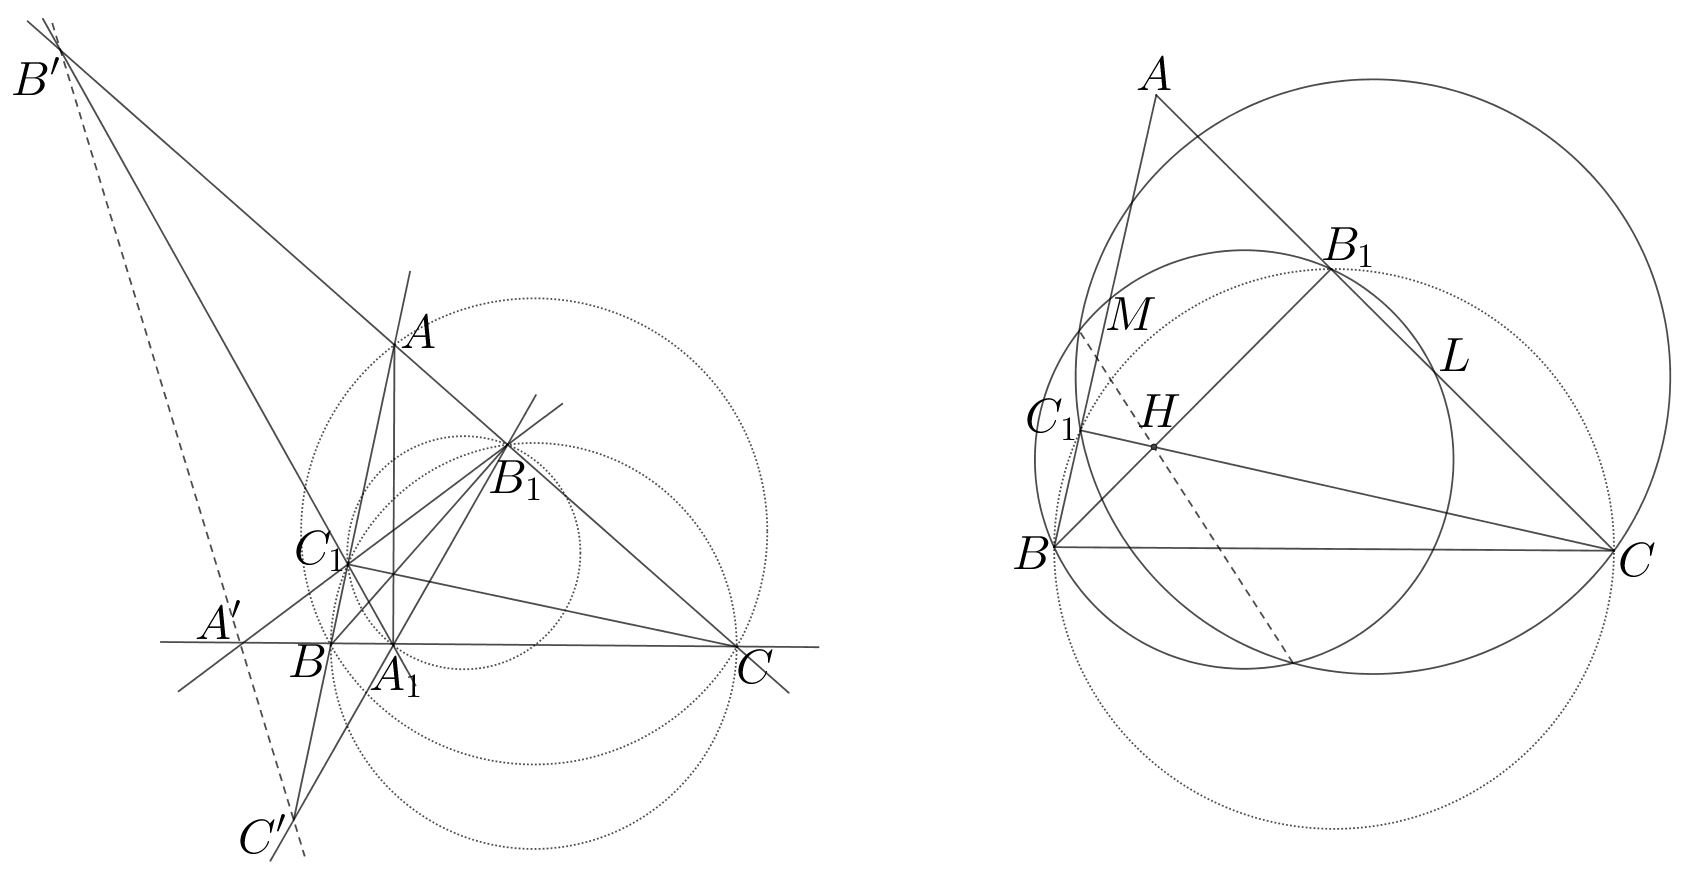
\includegraphics[scale=0.4]{Секретная информация/Решения листочков/axes-1.png}
        \caption{}\label{ris.axes-1}
    \end{center}
\end{figure}

\textbf{Решение. (a)} Рассмотрим окружности $(ABC)$ и $(A_1B_1C_1)$. Докажем, что точки $A'$, $B'$ и $C'$ лежат на их радикальной оси. Для этого рассмотрим окружность $(BCC_1B_1)$. Заметим, что прямая $B_1C_1$ является радикальной осью пары окружностей $(A_1B_1C_1)$ и $(BCC_1B_1)$, а прямая $BC$ --- радикальной осью пары окружностей $(ABC)$ и $(BCC_1B_1)$. Значит, точка $A'$ их пересечения является радикальным центром тройки окружностей $(ABC)$, $(BCC_1B_1)$ и $(A_1B_1C_1)$, а потому она лежит на радикальной оси окружностей $(ABC)$ и $(A_1B_1C_1)$. Рассуждения для точек $B'$ и $C'$ аналогичны.

{\bf (b)} Докажем, что общая хорда окружностей $\omega_b$ и $\omega_c$, построенных на отрезках $BL$ и $CM$ соответственно, проходит через $H$ (рассуждения для двух других хорд аналогичны). Рассмотрим окружность $(BCC_1B_1)$. Ясно, что точка $B_1$ лежит на окружности $\omega_b$, а точка $C_1$ --- на окружности $\omega_c$. Осталось заметить, что точка $H$ является радикальным центром трех окружностей $\omega_b$, $\omega_c$, $(BCC_1B_1)$, а потому общая хорда окружностей $\omega_b$ и $\omega_c$ действительно проходит через $H$, что и требовалось доказать.

\newpage

\hspace{3mm}

\problem{2} 
Для треугольника $ABC$ обозначим через $A_1$, $B_1$, $C_1$ основания высот. Пусть $A'$ --- точка пересечения касательных к окружности $(ABC)$ в точке $A$ и к окружности $(A_1B_1C_1)$ в точке $A_1$. Точки $B'$ и $C'$ определяются аналогично. Докажите, что точки $A'$, $B'$ и $C'$ лежат на одной прямой.

\begin{figure}[h]
    \begin{center}
        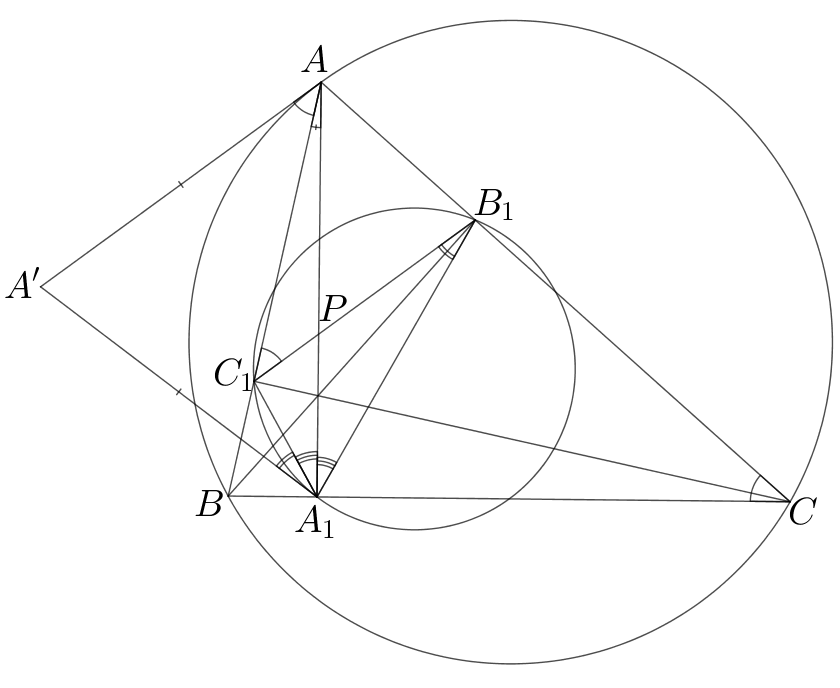
\includegraphics[scale=0.75]{Секретная информация/Решения листочков/axes-2.png}
        \caption{}\label{ris.axes-2}
    \end{center}
\end{figure}

\textbf{Решение.} Докажем, что отрезки $A'A$ и $A'A_1$ равны. Тогда точка $A'$ будет лежать на радикальной оси окружностей $(ABC)$ и $(A_1B_1C_1)$, а значит, точки $B'$ и $C'$ также будут лежать на этой оси. Посчитаем углы. Имеем: $$\angle A'AC_1=\angle ACB=\angle AC_1B_1, \quad \angle A'A_1C_1=\angle A_1B_1C_1, \quad \angle AA_1C_1=\angle AA_1B_1.$$ Наконец, $\angle A'AA_1=\angle A'AC_1+\angle A_1AC_1=\angle A_1AC_1+\angle AC_1B_1=\angle APB_1$ и $\angle A'A_1A=\angle A'A_1C_1+\angle C_1A_1A=\angle AA_1B_1+\angle A_1B_1C_1=\angle APB_1$. Таким образом, треугольник $A'AA_1$ равнобедренный и $A'A=A'A_1$, что и требовалось доказать.

\newpage

\hspace{3mm}

\problem{3}
К двум непересекающимся окружностям $\omega_1$ и $\omega_2$ проведены внешняя и внутренняя касательные $a$ и $b$, пересекающиеся в точке $C$. Обозначим точки касания окружностей $\omega_1$ и $\omega_2$ с прямой $a$ через $A_1$ и $A_2$, а с прямой $b$ --- через $B_1$ и $B_2$. Докажите, что прямые $A_1B_1$ и $A_2B_2$ пересекаются на линии центров окружностей $\omega_1$ и $\omega_2$.

\begin{figure}[h]
\begin{center}
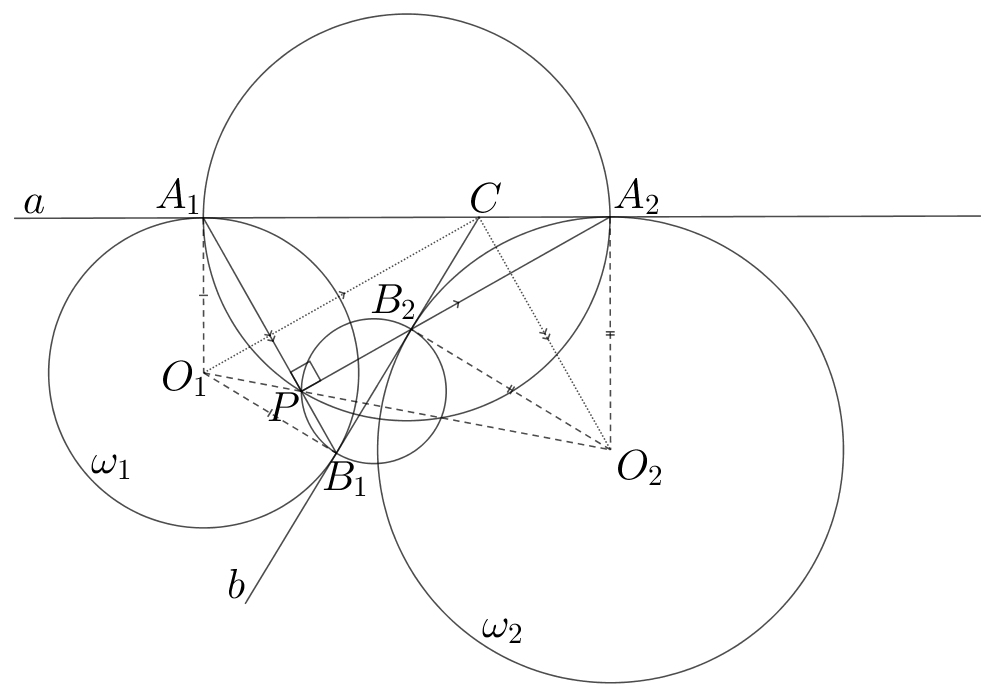
\includegraphics[scale=0.75]{Секретная информация/Решения листочков/axes-3.png}
\caption{}\label{ris.axes-3}
\end{center}
\end{figure}

\textbf{Решение.} Обозначим через $P$ точку пересечения прямых $A_1B_1$ и $A_2B_2$, а через $C$ --- точку пересечения прямых $a$ и $b$. Заметим, что прямые $O_1C$ и $A_2B_2$, а также прямые $O_2C$ и $A_1B_1$ попарно параллельны. Учитывая, что прямые $O_1C$ и $O_2C$ перпендикулярны, получаем, что $\angle A_1PA_2=90^\circ$. Рассмотрим окружности $(A_1A_2P)$ и $(B_1B_2P)$. Докажем, что прямая $O_1O_2$ явдяется их радикальной осью (тогда она должна проходить через точку $P$). Степень точки $O_1$ относительно окружности $(A_1A_2P)$ равна $O_1A_1^2$, поскольку отрезок $O_1A_1$ является касательной к окружности $(A_1A_2P)$. Аналогично, Степень точки $O_1$ относительно окружности $(B_1B_2P)$ равна $O_1B_1^2$. Но $O_1A_1=O_1B_1$, поэтому степени точки $O_1$ относительно обеих окружностей $(A_1A_1P)$ и $(B_1B_2P)$ равны. Рассуждения для точки $O_2$ совершенно аналогичны.

\newpage

\hspace{3mm}

\problem{4}  Вписанная окружность $\gamma$ треугольника $ABC$ касается его стороны $BC$ в точке $D$. Обозначим центр вневписанной в угол $A$ окружности через $I_a$, а середину отрезка $DI_a$ через $M$. Докажите, что отрезок касательной, проведённой из точки $M$ к $\gamma$, равен $MB$.

\begin{figure}[h]
\begin{center}
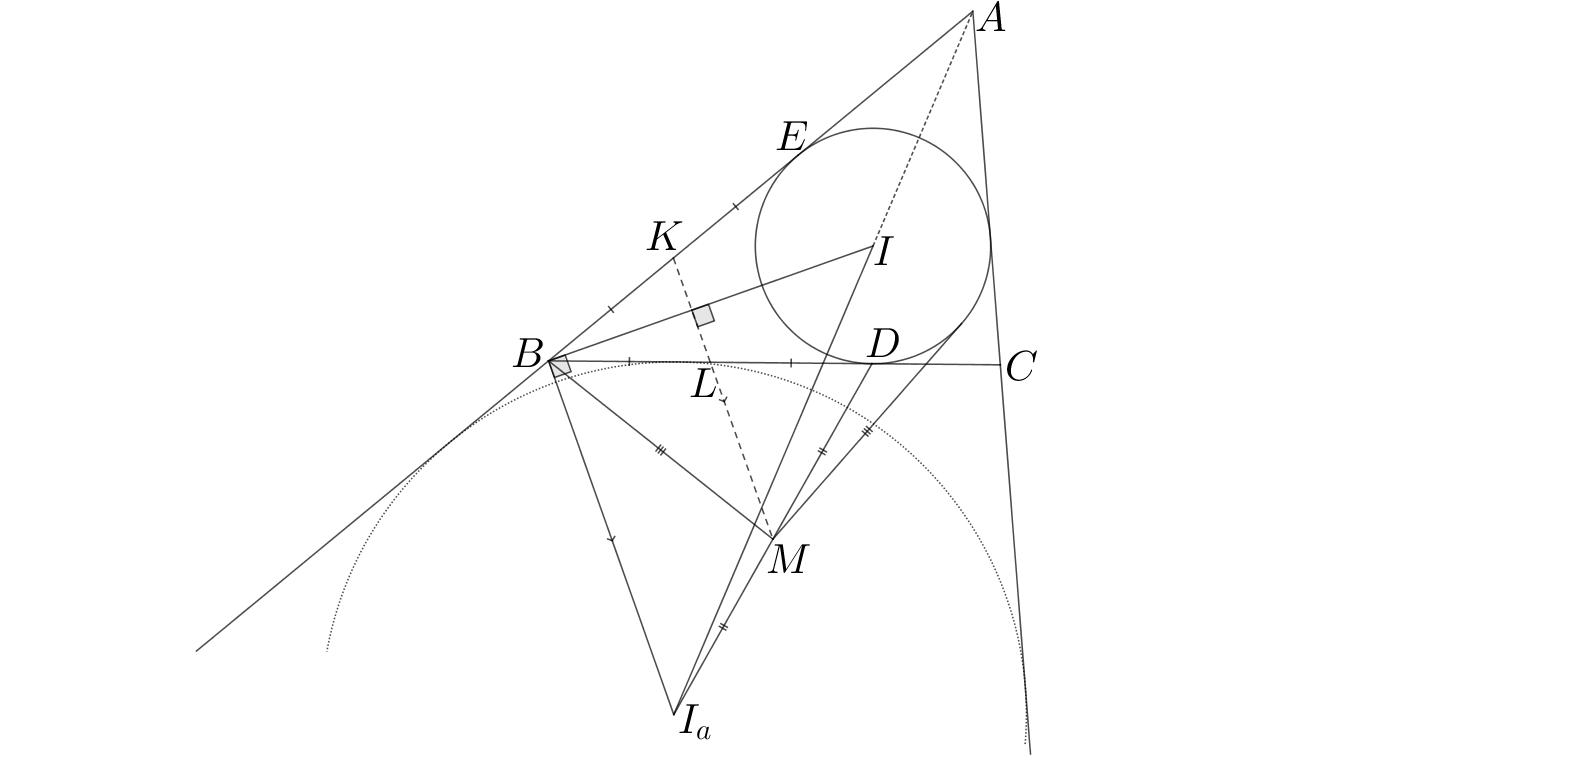
\includegraphics[scale=0.4]{Секретная информация/Решения листочков/axes-4.png}
\caption{}\label{ris.axes-4}
\end{center}
\end{figure}

\textbf{Решение.} Отметим центр $I$ вписанной окружности $\gamma$ треугольника $ABC$ и точку $E$ касания этой окружности со стороной $AB$. Докажем, что точка $M$ лежит на радикальной оси окружности $\gamma$ и точки $B$. Для этого рассмотрим середины $K$ и $L$ отрезков $BD$ и $BD$ и докажем, что точка $M$ лежит на прямой $KL$ (поскольку степени точек $K$ и $L$ относительно окружности $\gamma$ и точки $B$ равны, прямая $KL$ и будет нашей радикальной осью). Это совсем просто: прямая $KL$ перпендикулярна биссектрисе $BI$, а прямая $LM$ является средней линией треугольника $BDI_a$ и потому параллельна прямой $BI_a$, которая в свою очередь перпендикулярна $BI$. Значит, прямые $KL$ и $ML$ обе перпендикулярны прямой $BI$ и потому совпадают, что и требовалось доказать.

\newpage

\hspace{3mm}

\problem{5} 
К двум непересекающимся окружностям $\omega_1$ и $\omega_2$ проведены три общие касательные --- две внешние, $a$ и $b$, и одна внутренняя, $c$. Прямые $a$, $b$ и $c$ касаются окружности $\omega_1$ в точках $A_1$, $B_1$ и $C_1$ соответственно, а окружности $\omega_2$ --- в точках $A_2$, $B_2$ и $C_2$ соответственно. Докажите, что высоты треугольников $A_1B_1C_1$ и $A_2B_2C_2$, проведенные из вершин $C_1$ и $C_2$, равны.

\begin{figure}[h]
    \begin{center}
        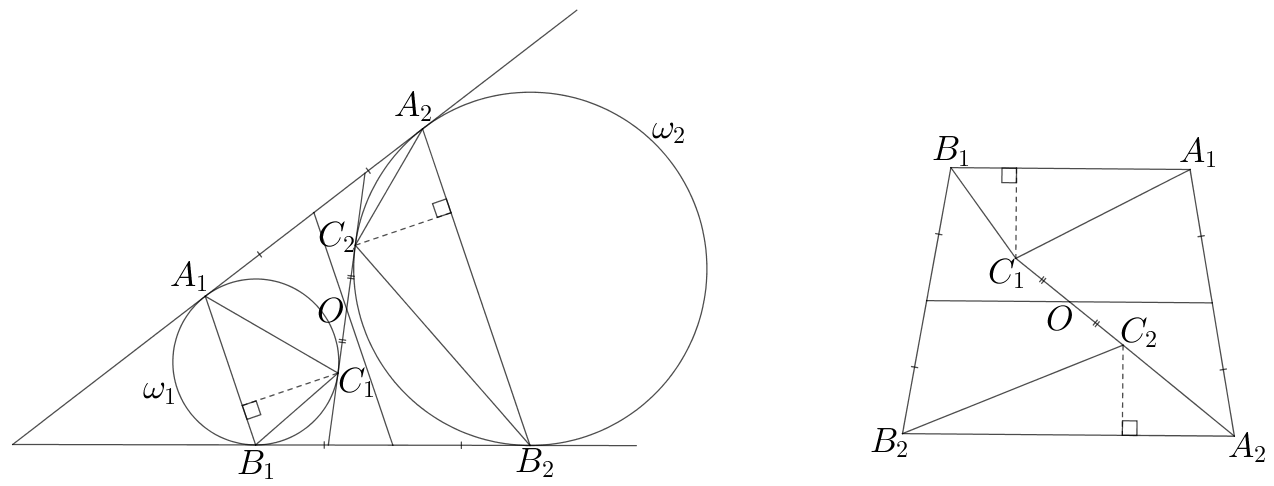
\includegraphics[scale=0.65]{Секретная информация/Решения листочков/axes-5.png}
        \caption{}\label{ris.axes-5}
    \end{center}
\end{figure}

\textbf{Решение.} Проведем радикальную ось окружностей $\omega_1$ и $\omega_2$. Пусть она пересекает прямую $c$ в точке $O$. Заметим, что четырехугольник $A_1B_1B_2A_2$ является равнобокой трапецией, средняя линия которой --- радикальная ось, а точка $O$ --- ее середина. Также $OC_1=OC_2$. Рассмотрим центральную симметрию $Z_O$ относительно точки $O$. Ясно, что $Z_O(C_1)=C_2$ и прямая $A_1B_1$ при такой центральной симметрии перейдет в прямую $A_2B_2$. Отсюда следует, что высота, опущенная из точки $C_1$ на прямую $A_1B_1$, перейдет в высоту, опущенную из точки $C_2$ на прямую $A_2B_2$. Значит, эти высоты равны, что и требовалось доказать.

\newpage

\hspace{3mm}

\problem{6}
Дан параллелограмм $ABCD$ с тупым углом $A$. Из точки $A$ на сторону $BC$ опущен перпендикуляр $AH$. Далее, в треугольнике $ABC$ из точки $C$ проведена медиана, продолжение которой пересекает окружность $(ABC)$ в точке $K$. Докажите, что точки $K$, $H$, $C$ и $D$ лежат на одной окружности.

\begin{figure}[h]
    \begin{center}
        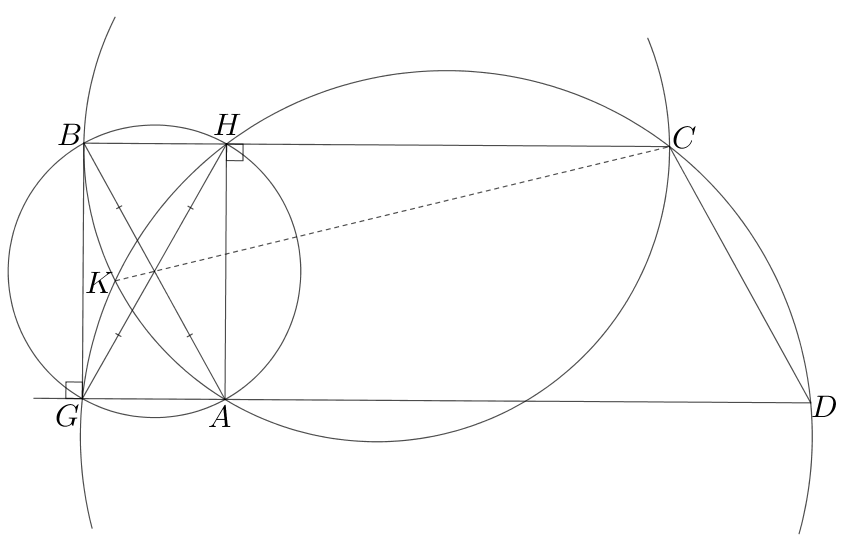
\includegraphics[scale=0.65]{Секретная информация/Решения листочков/axes-6.png}
        \caption{}\label{ris.axes-6}
    \end{center}
\end{figure}

\textbf{Решение.} Проведем перпендикуляр $BG$ из точки $B$ на прямую $AD$. Будем доказывать, что точка $K'$ пересечения окружностей $(ABC)$ и $(HCD)$, отличная от $C$, лежит на продолжении медианы треугольника $ABC$, проведенной из вершины $C$. Для этого рассмотрим окружности $(ABC)$, $(HCD)$ и $(ABH)$. Заметим, что четырехугольник $AHBG$ является прямоугольником, а четырехугольник $GHCD$ --- равнобокой трапецией, поэтому окружности $(HCD)$ и $(ABH)$ проходят через точку $G$. Значит, радикальные оси $AB$, $GH$ и $CK'$ окружностей $(ABC)$, $(HCD)$ и $(ABH)$ пересекаются в одной точке --- радикальном центре. Поскольку отрезки $AB$ и $GH$ являются диагоналями прямоугольника $AHBG$, радикальный центр является их серединами. Значит, точка $K'$ лежит на продолжении медианы треугольника $ABC$, проведенной из вершины $C$, и потому совпадает с точкой $K$, что и требовалось.

\newpage

\hspace{3mm}

\problem{7} Пусть $ABC$ --- неравнобедренный треугольник с ортоцентром $H$ и описанной окружностью $\Omega$. Прямая, проходящая через $H$, пересекает отрезки $AB$ и $AC$ в точках $E$ и $F$ соответственно. Пусть $K$ --- центр окружности $(AEF)$, и пусть прямая $AK$ вторично пересекает $\Omega$ в точке $D$. Докажите, что прямая $HK$ и прямая, проходящая через $D$ перпендикулярно $BC$, пересекаются на $\Omega$.

\begin{figure}[h]
\begin{center}
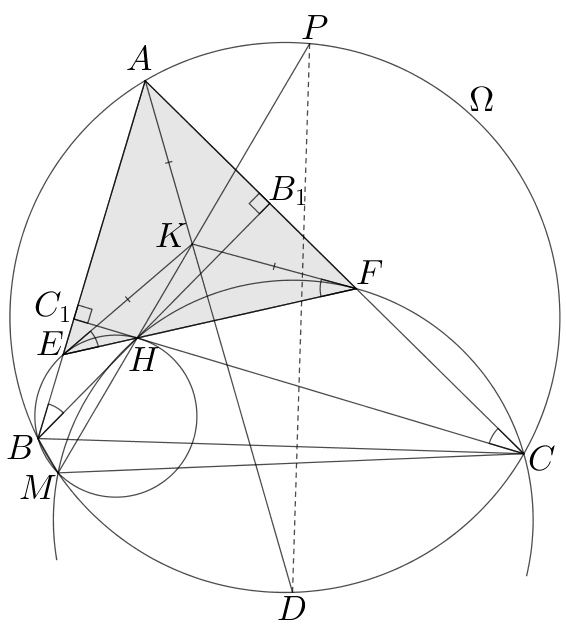
\includegraphics[scale=0.7]{Секретная информация/Решения листочков/axes-7.png}
\caption{}\label{ris.axes-7}
\end{center}
\end{figure}

\textbf{Решение.} Проведем высоты $BB_1$ и $CC_1$ в треугольнике $ABC$ и рассмотрим окружности $(BEH)$ и $(CFH)$. По теореме Микеля для треугольника $AEF$ эти окружности вторично пересекаются в точке $M$, лежащей на окружности $\Omega$. Далее, заметим, что отрезок $KE$ является касательной к окружности $(BEH)$, т.к. $\angle KEF=90^\circ-\angle EKF/2=90^\circ-\angle A=\angle EBH$. Аналогично, отрезок $KF$ является касательной к окружности $(CFH)$. Поскольку эти отрезки равны, то точка $K$ лежит на радикальной оси окружностей $(BEH)$ и $(CFH)$, т.е. на прямой $MH$. 

Пусть $P$ --- вторая точка пересечения прямой $MH$ и окружности $\Omega$. Докажем, что прямые $PD$ и $BC$ перпендикулярны. Для этого посчитаем угол между хордами $BC$ и $DP$ в окружности $\Omega$. Он равен $$\angle PMC+\angle BAD=\angle AFE+\angle EAK=90^\circ,$$ что и требовалось.